\subsection{Абстрактный синтаксис}
Описание языка в среде \MPS{} обычно начинается с задания абстрактного синтаксиса \cite{redDragon} этого языка. Для этого в среде \MPS{} предусмотрен специальный проблемно-ориентированный язык \term{jetbrains.mps.bootstrap.structureLangauge} (далее \term{structureLanguage}). Этот язык позволяет описать концепты языка и отношения между ними. С помощью этого же языка задаются свойства и мета-свойства концептов. Весь абстрактный синтаксис языка описывается в модели \term{structure} этого языка.

Для объявления пользовательских концептов в языке \term{structureLangauge} определен концепт \term{ConceptDeclaration}. Например, корневой узел, описывающий концепт \term{StateMachine}, предствлен на рисунке \ref{fig:StateMachineConcept}.

\begin{figure}
\centering
\fbox{
 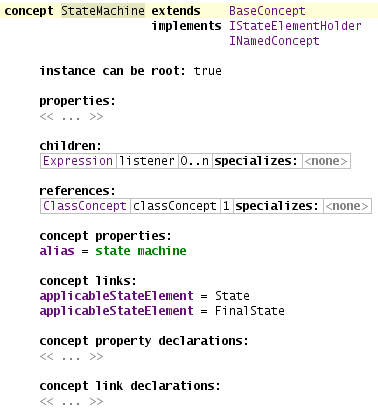
\includegraphics[width=0.9\textwidth]{StateMachineConcept.png}
}
\caption{Объявление концепта \term{StateMachine}}
\label{fig:StateMachineConcept}
\end{figure}


Из рисунка видно, что объявление концепта состоит из нескольких секций:
\begin{itemize}
 \item секция \term{concept StateMachine} задает имя концепта;

 \item секция \term{extends BaseConcept} указывает на то, что концепт является расширением концепта \term{BaseConcept}.
 Отношение расширения в языке \term{structureLanguage} имеет тот же смысл, что и в традиционных объектно-ориентированных
 языках программирования: если концепт \term{B} является расширением концепта \term{A}, то все экземпляры концепта \term{B}
 являются также и экземплярами концепта \term{A}. Так же концепт \term{B} наследует все свойства и отношения концепта
 \term{A}.  Каждый концепт объявленный в среде \MPS{} является прямым или косвенным расширением концепта
 \term{BaseConcept},  также как в языке \term{Java} все классы прямо или косвенно расширяют класс \term{java.lang.Object};

 \item в секции \term{implements IStateElementHolder INamedConcept} перечислены интерфейсы-концепты реализуемые
 концептом \term{StateMachine}. Понятие \term{интерфейса-концепта} ближе всего к понятию \term{trait} языка \term{Scala} [ссылка].
 Интерфейс-концепт также может иметь свойства и отношения с другими концептами. При этом не может быть узлов,
 являющихся непосредственными экземплярами интерфейса-концепта. Интерфейсы-концепты полезны для создания неполного
 множественного наследования: концепт наследует все свойства и отношения тех интерфейсов-концептов, которые он
 реализует;

 \item в секции \term{instance can be root} задается могут ли экземпляры концепта быть корневыми узлами моделях. В
 данном случае, экземпляры концепта \term{StateMachine} могут быть корневыми;

 \item в секции \term{properties} перечисляются свойства, которые может иметь экземпляр концепта. Концепт \term{StateMachine} не определяет собственных свойств, однако у экземпляров этого концепта может быть задано свойство \term{name}, унаследованное от интерфейса-концепта \term{INamedConcept};

 \item в секции \term{children} описывается структура вложенных узлов. Для каждого элемента в этой секции задается концепт, роль и арность вкладываемых узлов. Арность определяет ограничение на количество вложенных экземпляров данного концепта с данной ролью. Арность может быть задана одним из четырех значений:
\begin{description}
 \item["<1">] ровно один экземпляр;
 \item["<0..1">] не более одного экземпляра;
 \item["<1..n">] хотя бы один экземпляр;
 \item["<0..n">] произвольное количество экземпляров.
\end{description}
Например, в экземпляр концепта \term{StateMachine} может быть вложено произвольное количество экземпляров концепта \term{Expression} с ролью \term{listener}. Кроме этого экземпляр концепта \term{StateMachine} может содержать произвольное количество вложенных экземпляров интерфеса-концепта \term{IStateElement}, так как в секции \term{children} интерфейса-концепта \term{IStateElementHolder} есть элемент \term{IStateElement stateElement 0..n}, и концепт \term{StateMachine} реализует интерфейс-концепт \term{IStateElementHolder};

\item в секции \term{references} определяется структура ссылок концепта. Также, как и в случае вложенных узлов, каждый элемент в этой секции задает целевой концепт, роль и арность ссылки. Арность ссылки может быть задана одним из двух значений:
\begin{description}
 \item["<1">] обязательная ссылка;
 \item["<0..1">] необязательная ссылка.
\end{description}
Например, каждый экземпляр концепта \term{StateMachine} должен иметь ссылку с ролью \term{classConcept} на экземпляр концепта \term{ClassConcept};

\item четыре последних секции предназначены для описания мета-структы концепта. в секции \term{concept properties} задаются значения мета-свойства концепта. Для концепта \term{StateMachine} значение мета-свойства \term{alias} определено как \term{state machine}. Это специальное мета-свойство, значение которого используется средой \MPS{} в качестве имени концепта в пользовательском интерфейсе. Например, в меню создания корневого узла, опция, соответствующая созданию экземпляра концепта \term{StateMachine}, будет называться \term{state machine} (Рис. \ref{fig:CreateStateMachine}).

\begin{figure}
 \centering
 \fbox{
  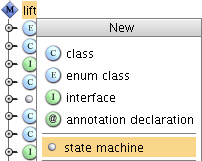
\includegraphics{CreateStateMachine.png}
 }
 \caption{Меню создания корневого узла}
 \label{fig:CreateStateMachine}
\end{figure}

В секции \term{concept links} задаются значения мета-отношений концепта. В секциях \term{concept property declaration} и \term{concept link declarations} объявляются мета-свойства, значения которых могут быть заданы в самом концепте или в расширяющих его концептах. Например, в интерфейсе-концепте \term{IStateElementHolder} объявлено мета-отношение \term{applic\-able\-Sta\-te\-Ele\-ment}, значение которого используется в языке \term{stateMachine} для того, чтобы уточнить какие именно автоматные конструкции могут быть вложены в другие автоматные конструкции. Значения
$$
\begin{array}{l}
applicableStateElement = State\\
applicableStateElement = FinalState
\end{array}
$$
для концепта \term{StateMachine} указывают на то, что автомат может содержать обычные и конечные состояния.
\end{itemize}

Абстрактный синтаксис языка может быть представлен виде UML-диаграммы классов \cite{uml}. Для языка \term{stateMachine} такая диаграмма приведена на рисунке \ref{fig:AbstractSyntax}.

\begin{figure}
 \centering
 \fbox{
  
\includegraphics{AbstractSyntax.png}
 }
 \caption{Абстрактный синтаксис языка \term{stateMachine}}
 \label{fig:AbstractSyntax}
\end{figure}
